% Source: graduate-coursework/Sp26/CSCE775/HW1/HW1_CSCE_775.tex

\documentclass[border=4pt]{standalone}
\usepackage{amsmath}
\usepackage{amssymb}
\usepackage{bm}
\usepackage{graphicx}
\usepackage{pgfplots}
\usepackage{tikz}
\usepackage{xcolor}
\pgfplotsset{compat=1.18}
\usetikzlibrary{shapes.geometric, arrows.meta, positioning, automata, calc, decorations.markings, patterns}

\definecolor{USC_Garnet}{HTML}{73000A}
\definecolor{USC_Sandstorm}{HTML}{FFF2E3}
\definecolor{USC_Black90}{HTML}{363636}
\definecolor{USC_Black70}{HTML}{5C5C5C}
\definecolor{USC_Black50}{HTML}{A2A2A2}
\definecolor{USC_Black10}{HTML}{ECECEC}
\definecolor{USC_Honeycomb}{HTML}{A49137}
\definecolor{USC_Horseshoe}{HTML}{65780B}
\definecolor{USC_Atlantic}{HTML}{466A9F}
\definecolor{USC_Congaree}{HTML}{1F414D}
\definecolor{USC_Rose}{HTML}{CC2E40}


\begin{document}
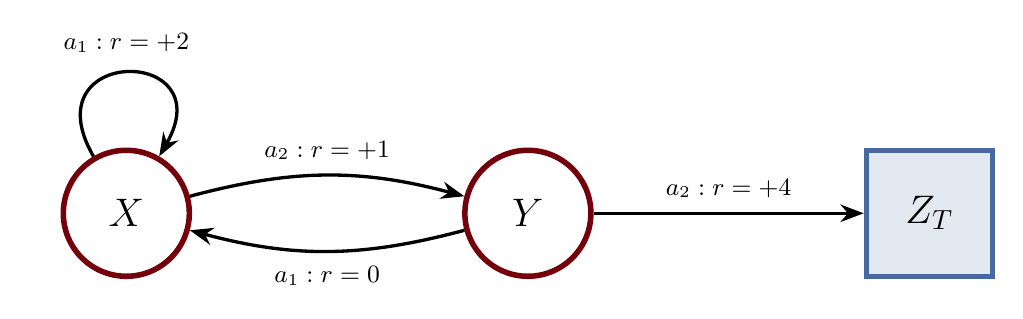
\begin{tikzpicture}[
    >=Stealth,
    scale=0.85,
    every state/.style={
        fill=white,
        draw=USC_Garnet,
        line width=2pt,
        text=black,
        minimum size=1.6cm,
        font=\bfseries\Large
    },
    every edge/.style={draw=black, line width=1.2pt, ->, >=Stealth},
    prob/.style={font=\small\bfseries, fill=white, inner sep=2pt},
    term/.style={
        fill=USC_Atlantic!15,
        draw=USC_Atlantic,
        line width=2pt,
        text=black,
        minimum size=1.6cm,
        font=\bfseries\Large
    }
]

\node[state] (X) at (0, 0) {$X$};
\node[state] (Y) at (6, 0) {$Y$};
\node[term] (Z) at (12, 0) {$Z_T$};

% X actions
\path (X) edge[loop above, looseness=5, out=120, in=60] node[prob, above=5pt] {$a_1: r=+2$} (X);
\path (X) edge[bend left=15] node[prob, above=3pt] {$a_2: r=+1$} (Y);

% Y actions
\path (Y) edge[bend left=15] node[prob, below=3pt] {$a_1: r=0$} (X);
\path (Y) edge node[prob, above=3pt] {$a_2: r=+4$} (Z);

\end{tikzpicture}
\end{document}
